\chapter{Flyback Switching Power Supply for Battery Charger}
The goal is to use the circuit shown in the following figure to create a 24V battery charger.

\begin{figure}[h]
\centering
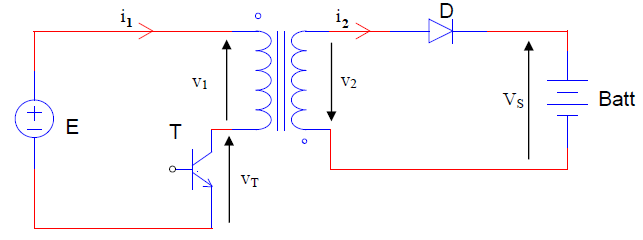
\includegraphics[width=0.9\linewidth]{TD_Flyback/fig/FlybackBatterie.png}
\end{figure}

Let $n_1$ and $n_2$ be the respective numbers of turns in the primary and secondary windings, with the transformation ratio denoted as $m$. The primary magnetizing inductance is denoted as $L_1$, the switching frequency as $f$, and the duty cycle as $\alpha$.

The initially discharged battery has a voltage of $V_{S0} = 20V$ across its terminals. The charging process will be stopped when the voltage across the terminals reaches $V_{S1} = 26V$. However, throughout the analysis, this battery voltage, denoted as $V_S$, will be assumed to be constant on the timescale of the switching.

At the beginning of the battery charging process, it is assumed that the power supply operates in critical mode with a duty cycle of $\alpha_0$, and the average current in the battery is $I_{S0}$.

\vspace{0.25cm}
Numerical values: $E = 300V$; $f = 20 kHz$; $\alpha_0 = 0.5$; $I_{S0} = 10 A$.

\begin{enumerate}

\item \textbf{Start of charging}
\begin{enumerate}
\item Provide the expression of Hopkinson's theorem relating $n_1$, $i_1$, $n_2$, $i_2$, and $R$ (reluctance of the ferrite core, inverse of the specific inductance $A_L$), and $\varphi$ (elementary flux in the core).
\item Plot the waveforms of $i_1$, $i_2$, $\varphi$, $v_T$, and $v_1$ over one switching period.
\item Deduce the expression of the output voltage $V_S$ in terms of $E$, $m$, and $\alpha_0$. Calculate the numerical value of $m$.
\item Determine the expression of the average output current $I_{S0}$ in terms of $L_1$, $\alpha_0$, $m$, $E$, and $f$. Calculate the numerical value of $L_1$.
\item Calculate the energy $W_D$ delivered to the battery per switching cycle using two different methods.
\item Calculate the numerical value of this energy $W_D$ and determine the charging time at constant current for a battery with a "capacity" of 25 Ah.
\end{enumerate}
\item \textbf{End of charging}

During the charging process, the output voltage slowly increases from $V_{S0}$ to $V_{S1}$ while maintaining the duty cycle at $\alpha_0$.
\begin{enumerate}
\item How has the conduction mode of the power supply been modified?
\item Plot the waveforms of $i_1$, $i_2$, $v_T$, and $v_1$ over one switching period.
\item What is the conduction time of the diode D?
\item What is the energy transferred per cycle now? Determine the average current $I_S$ supplied to the battery.
\item What value $\alpha_1$ should be given to the duty cycle to subsequently provide an average charging current of $I_{S1} = I_{S0}/10$?
\end{enumerate}

\item \textbf{Saturation limit}

We are in the critical mode (start of charging).

\begin{enumerate}
\item Determine the expression of the maximum magnetic induction in the ferrite core in terms of $E$, $\alpha$, $T$, $n_1$, and $A_e$ (effective area of the core).
\item Deduce the expression of the minimum value $A_{e\ min}$ of the core area to prevent any saturation of the material. For this purpose, let $B_{sat}$ be the induction value near saturation.
\end{enumerate}

\item \textbf{Winding window area}

We are still in the critical mode (start of charging).

\begin{enumerate}
\item Using the results from the first part, determine the effective value $I_{1\ eff}$ of the current in the transistor in terms of the output current $I_s$, $m$, and $\alpha$.
\item Similarly, express the effective value $I_{2\ eff}$ of the secondary current in terms of $I_s$ and $\alpha$.
\item The chosen current density for both windings made of copper wire is $\delta$. Determine the expression of the total copper area, denoted as $S_{T\ Cu}$, in terms of $I_s$, $\delta$, $n_2$, and $\alpha$. Compare the primary and secondary copper areas.
\item Deduce the minimum winding window area, denoted as $S_B$, if a winding coefficient $k_B$ is chosen ($S_{T\ Cu} = k_B.S_B$).
\end{enumerate}

\item \textbf{Choice of magnetic core}

\begin{enumerate}
\item Based on the results from the previous questions, determine the inequality that the product $A_e.S_B$ of this power supply must satisfy in terms of $B_{sat}$, $P_s$, $T$, $k_B$, $\delta$, and $\alpha$.
\item Calculate the minimum value of this product in $mm^4$ for the following numerical values:

\begin{center}
$P_s = 200 W$; $\alpha = 0.5$; $k_B = 0.5$; $B_{sat} = 0.4 T$; $\delta = 5 A.mm^{-2}$; $f = 20 kHz$.
\end{center}

\item Choose a core from the following list, for which the manufacturer provides the values of $A_e$, $S_B$, and $A_L$ (specific inductance) without air gap, as well as $A_L$ with a 0.5 mm air gap. Note that all these cores are made of the same material, N41.

\vspace{1mm}
\begin{tabular}{| c | c | c | c | c |}
	\hline
	\multirow{2}*{Core} & \multirow{2}*{$A_e\ (mm^2)$} & \multirow{2}*{$S_B \ (mm^2)$} & $A_L$ without air gap & $A_L$ with 0.5 mm air gap\\
	 & & & (nH) & (nH)\\
	\hline
	%RM4 & 11 & 14 & 63 & - - - \\
	\hline
	RM6 & 31 & 32 & 3100 & - - -\\
	\hline
	RM8 & 55 & 57 & 4100 & 160\\
	\hline
	RM10 & 90 & 93 & 5500 & 250\\
	\hline
	RM12 & 125 & 128 & 6000  & 300 \\
	\hline
	RM14 & 170 & 176 & 6800 & 400 \\
	\hline
\end{tabular}

\vspace{1mm}


\item For this choice of core, determine the minimum numbers of turns $n_1$ and $n_2$ to limit the maximum induction in the ferrite core to $B_{sat}$. For these calculations, choose the values of the numbers of turns that are "optimal" for the given numerical values.

\item Will an air gap be necessary to achieve the desired inductance $L_1$?

\end{enumerate}

\begin{figure}[h]
\centering
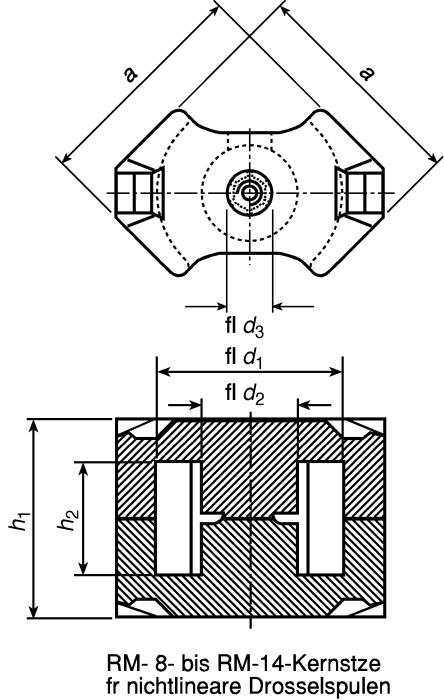
\includegraphics[width=0.5\linewidth]{TD_Flyback/fig/noyau.png}
\end{figure}

\end{enumerate}
